\documentclass[landscape]{article}

\pagenumbering{gobble}
\usepackage{tikz}
\usetikzlibrary{calc,shapes,positioning}
\usetikzlibrary{arrows}
\newcommand{\midarrow}{\tikz \draw[-triangle 90] (0,0) -- +(.1,0);}
\usepackage{bm}
\newcommand{\Ss}{\mathcal{S}}
\newcommand{\Tt}{\mathcal{T}}

\usepackage{amsmath,graphicx}
\newcommand{\ubar}[1]{\mkern2mu\underline{\mkern-2mu #1\mkern-2mu}\mkern2mu}
\newcommand{\ubm}[1]{\ubar{\bm{#1}}}
% \newcommand{\ubmr}[2]{\ubar{\bm{#1}}^{#2}}

\begin{document}

\begin{figure}

  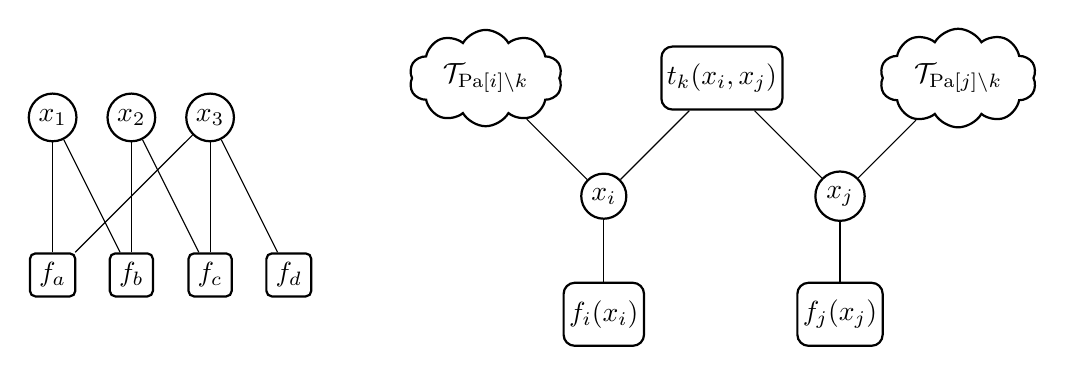
\begin{tikzpicture}
    \begin{scope}[xshift=-2cm]
      \tikzstyle{enode} = [thick, draw=black, circle, inner sep = 2pt,  align=center]
      \tikzstyle{nnode} = [thick, rectangle, rounded corners = 2pt, minimum size = 0.5cm,draw]
      \begin{scope}[yshift=1cm]
        \node[enode] (x1) at (-1.5, 1) {$x_1$};
        \node[enode] (x2) at (-0.5, 1) {$x_2$};
        \node[enode] (x3) at (0.5, 1) {$x_3$};
      \end{scope}
      \node[nnode] (a) at (-1.5,0) {$f_a$};
      \node[nnode] (b) at (-0.5,0) {$f_b$};
      \node[nnode] (c) at (0.5,0) {$f_c$};
      \node[nnode] (d) at (1.5,0) {$f_d$};

      \draw[-] (a) to (x1);
      \draw[-] (a) to (x3);
      \draw[-] (b) to (x1);
      \draw[-] (b) to (x2);
      \draw[-] (c) to (x2);
      \draw[-] (c) to (x3);
      \draw[-] (d) to (x3);
    \end{scope}


    \begin{scope}[xshift=5cm, yshift=1cm]
      \tikzstyle{enode} = [thick, draw=black, circle, inner sep = 2pt,  align=center]
      \tikzstyle{nnode} = [thick, rectangle, rounded
      corners = 4pt, minimum size = 0.8cm,draw,inner sep = 2pt]

      \tikzstyle{cnode} = [thick, cloud, draw,
      cloud puffs=10, cloud puff arc=120, aspect=2, inner ysep=4pt]

      \node[cnode] (pajk) at (3, 1.5) {$\Tt_{\text{Pa}[j]\backslash k}$};
      \node[cnode] (paik) at (-3, 1.5) {$\Tt_{\text{Pa}[i]\backslash k}$};

      \node[nnode] (tk) at (0, 1.5) {$t_k(x_i, x_j)$};
      \node[enode] (xi) at (-1.5 ,0) {$x_i$};
      \node[nnode] (fi) at (-1.5 , -1.5) {$f_i(x_i)$};

      \node[enode] (xj) at (1.5 ,0) {$x_j$};
      \node[nnode] (fj) at (1.5 , -1.5) {$f_j(x_j)$};
      % connections

      \draw[-] (xi) to (fi);
      \draw[-] (xi) to (tk);
      \draw[-] (xi) to (paik);

      \draw[-] (xj) to (fj);
      \draw[-] (xj) to (tk);
      \draw[-] (xj) to (pajk);
    \end{scope}

  \end{tikzpicture}


\end{figure}


\end{document}
%%% Local Variables:
%%% mode: latex
%%% TeX-master: t
%%% End:
